\documentclass[a4paper,10pt]{article}

%\VignetteIndexEntry{PREDA tutorial}

\usepackage[latin1]{inputenc}
\usepackage[english]{babel}
\usepackage{fontenc}
\usepackage{graphicx}

\title{PREDA tutorial}

\usepackage{Sweave}
\begin{document}
\maketitle

\begin{abstract}

PREDA (Position RElated Data Analysis) tool is a novel R package for integrative analyses of functional genomics data. PREDA implements a procedure to analyze the relationships between data and physical genomic coordinates along chromosomes with the final aim of identifying chromosomal regions with likely relevant functional role.
The procedure for position related data analysis is highly flexible and can be applied on data obtained with different technologies. In principle, it can analyze different types of quantitative functional genomics data, e.g., gene expression, copy number, methylation levels. In particular, the underlying algorithm so far has been successfully adopted for the analysis of gene expression and copy number data obtained with various microarray platforms on different organisms. This tool can also integrate analysis results from different types of functional genomics data (e.g. integrated analysis of copy number and gene expression).

\end{abstract} 

\newpage

\tableofcontents

\newpage


\section{PREDA overview}

The relationships between gene expression and genomics coordinates can be addressed as a regression problem as firstly proposed by Toedling et al. \cite{PubMed_15572464}. A further refinement of this concept was proposed by Callegaro et Al. \cite{PubMed_16951291} adopting a method based on non linear kernel regression with adaptive bandwidth, so as to affectively take into account the extreme variability in data density along the genome: LAP (Locally Adaptive Procedure). This method was subsequently further extended in order to address different biological problems, considering different organisms, and different types of data and high throughput technologies \cite{PubMed_17683550,PubMed_18039355,PubMed_19542187,PubMed_19059999,PubMed_19615122}.
PREDA implements these methodologies in a flexible framework thus allowing its adoption in a broad spectrum of genomics studies. The potential utilizations cover the study of physiological mechanisms affecting genome utilization, such as cellular differentiation, as well as the study of pathological processes involving genome structure modifications, such as chromosomal translocations in cancer. See also the supplementary material about PREDA method for more details about the analysis algorithm.


\paragraph{Core of the underlying algorithm.} The core of the underlying algorithm is an improved version of the LAP procedure \cite{PubMed_16951291} which consists of three main steps:
\begin{enumerate}
 \item computation of a statistic on each gene (or other genomic features);
 \item non linear regression for smoothing the statistic along genomic coordinates;
 \item permutations of gene related statistics followed by smoothing to empirically estimate the local significance of observed smoothed statistics along the genome.
\end{enumerate}



\paragraph{Key features.} The method characteristics allow the adoption of the method for position related analysis in a broad variety of applications. In principle, PREDA can be adopted for the analysis of high throughput genomic data obtained with different technologies. Moreover, it can analyze different types of quantitative functional genomics data, e.g., gene expression, copy number, methylation levels. Some of its key features improving the method flexibility are:
\begin{itemize}
 \item Smoothing method accounting for variable density in genomics data
 \item No assumptions on the distribution of genes (or other genomic features)
 \item No assumptions on the distribution of statistics computed on genes (or other genomic features)
 \item Different scores can be adopted for different applications
 \item Data from different technologies can be adopted
\end{itemize}


\paragraph{Modular framework.} The basic computational framework can be easily further extended if custom analytical pipelines are required for more complex or specialized purposes. Custom S4-classes have been defined to manage data and genomic information required for the analyses thus facilitating further implementation of custom analytical workflows. See also the vignette about PREDA S4-classes.


\paragraph{Parallel computing.} Since the analytical procedure is time consuming, a parallelized version of the algorithm has been also implemented, based on Rmpi, to speed up the analyses. The parallel implementation allows to take advantage both of High Performance Computing systems and of modern multi-core processors that are currently available in common desktop computers.



\section{PREDA step by step}
The first part of PREDA tutorial is focused on a sample analysis aiming at identifying differentially expressed genomic regions. The PREDA analysis workflow is described taking into account every individual step of the analysis. In subsequent sections some wrapper functions performing the whole analyis with one single command will be describe as well. The adoption of wrapper functions certainly constitute a simpler and more user friendly solution for PREDA analysis. Nevertheless it's worth describing more in details what's going on in the background of each PREDA step.

\paragraph{Sample gene expression dataset.} Gene expression microarray data from a previously described dataset \cite{PubMed_19542187,PubMed_18194544} concerning clear renal cell carcinoma (RCC) and normal kidney cell samples are used in the following analysis. In particular this dataset is constituted by a subset of samples derived from ArrayExpress dataset E-TABM-282: the same subset used for the analyses described in \cite{PubMed_19542187}. The sample gene expression dataset includes 12 samples of clear cell renal carcinoma and 11 samples from normal kidney tissue. The table \ref{tab:Samplegeneexpressiondataset} reports the complete list of selected samples including sample classes, sample names adopted in the following analyses and original raw data files names (.CEL files) that are freely available for download from ArrayExpress repository. The same table is reported in the tab delimited TXT file (\texttt{sampleinfoGE\_PREDA.txt}) used to collect samples information.


\begin{table}[hbt]
 \centering
\begin{tabular}{ | l | r | r |}
\hline
Arrayname & Samplename & Class \\
\hline
27CG\_03i16741\_K\_Two\_Cycle\_IVT\_06mar06.CEL & 27CG & RCC \\
\hline
28RA\_04i3579\_K\_Two\_Cycle\_IVT\_06mar06.CEL & 28RA & RCC \\
\hline
33K\_04i13776\_Two\_Cycle\_IVT\_27oct05.CEL & 33BV & RCC \\
\hline
36K\_04i18916Two\_Cycle\_IVT\_27oct05.CEL & 36MML & RCC \\
\hline
37K\_04i19473\_Two\_Cycle\_IVT\_12.10.05.CEL & 37BA & RCC \\
\hline
40K\_04i20257\_Two\_Cycle\_IVT\_27oct05.CEL & 40RR & RCC \\
\hline
45DM\_05i5902\_K\_Two\_Cycle\_IVT\_25gen06.CEL & 45DM & RCC \\
\hline
46SA\_05i6348\_K\_Two\_Cycle\_IVT\_26gen06.CEL & 46SA & RCC \\
\hline
47CA\_04i3579\_K\_Two\_Cycle\_IVT\_06mar06.CEL & 47CA & RCC \\
\hline
49CA\_05i6348\_K\_Two\_Cycle\_IVT\_25gen06.CEL & 49CA & RCC \\
\hline
50PC\_05i9837\_K\_Two\_Cycle\_IVT\_06mar06.CEL & 50PC & RCC \\
\hline
51MI\_05i10081\_K\_Two\_Cycle\_IVT\_26gen06.CEL & 51MI & RCC \\
\hline
28RA\_04i3579\_C\_Two\_Cycle\_IVT\_06mar06.CEL & Norm1 & normal \\
\hline
32GM\_04i12879\_C\_Two\_Cycle\_IVT\_25gen06.CEL & Norm2 & normal \\
\hline
33N\_04i13776\_Two\_Cycle\_IVT\_27oct05.CEL & Norm3 & normal \\
\hline
35PA\_04i18143\_C\_Two\_Cycle\_IVT\_25gen06.CEL & Norm4 & normal \\
\hline
36N\_04i18916Two\_Cycle\_IVT\_27oct05.CEL & Norm5 & normal \\
\hline
37N\_04i19473\_Two\_Cycle\_IVT\_12.10.05.CEL & Norm6 & normal \\
\hline
40N\_04i20257\_Two\_Cycle\_IVT\_27oct05.CEL & Norm7 & normal \\
\hline
41SG\_04i20655\_C\_Two\_Cycle\_IVT\_26gen06.CEL & Norm8 & normal \\
\hline
44DE\_05i3989\_C\_Two\_Cycle\_IVT\_25gen06.CEL & Norm9 & normal \\
\hline
50PC\_05i9837\_C\_Two\_Cycle\_IVT\_26gen06.CEL & Norm10 & normal \\
\hline
51MI\_05i10081\_C\_Two\_Cycle\_IVT\_26gen06.CEL & Norm11 & normal \\
\hline
\end{tabular}
 \caption{Sample gene expression dataset: samples derived from ArrayExpress dataset E-TABM-282.}
 \label{tab:Samplegeneexpressiondataset}
\end{table}



First of all we have to load the required libraries: PREDAsampledata, providing the sample dataset and the PREDA package.


\begin{Schunk}
\begin{Sinput}
> require("PREDAsampledata")
> require("PREDA")
\end{Sinput}
\end{Schunk}

Then the variables defining the path to the directory containing the raw CEL files is defined, as well as the path to the sampleinfo file containing in a tab delimited TXT file the same information reported in table \ref{tab:Samplegeneexpressiondataset}. The information from the infofile are loaded into R with a \texttt{read.table()} command. The use of an ``infofile'' to hold information abut samples (raw data file, samplename and sample classes) is a very common solution for microarray data analysis, therefore the same convention is adopted here.

\begin{Schunk}
\begin{Sinput}
> CELfilesPath <- system.file("sampledata", "GeneExpression", 
+     package = "PREDAsampledata")
> infofile <- file.path(CELfilesPath, "sampleinfoGE_PREDA.txt")
> sampleinfo <- read.table(infofile, sep = "\t", 
+     header = TRUE)
> head(sampleinfo)
\end{Sinput}
\begin{Soutput}
                                  Arrayname Samplename
1 27CG_03i16741_K_Two_Cycle_IVT_06mar06.CEL       27CG
2  28RA_04i3579_K_Two_Cycle_IVT_06mar06.CEL       28RA
3    33K_04i13776_Two_Cycle_IVT_27oct05.CEL       33BV
4     36K_04i18916Two_Cycle_IVT_27oct05.CEL      36MML
5   37K_04i19473_Two_Cycle_IVT_12.10.05.CEL       37BA
6    40K_04i20257_Two_Cycle_IVT_27oct05.CEL       40RR
  Class
1   RCC
2   RCC
3   RCC
4   RCC
5   RCC
6   RCC
\end{Soutput}
\end{Schunk}



\subsection{Input data}
This sample analysis aims at identifying differentially expressed genomic regions in a group of tumor samples (clear cell renal carcinoma - RCC) when compared with a group of normal kidney cell samples. The input data is constituted by the raw gene expression data from Affymetrix GeneChip described above. Raw Affymetrix GeneChips data files (.CEL files) can be preprocessed in R using Bioconductor libraries: see also the Bioconductor documentation for further details, and in particular the documentation for package affy. In this sample analysis the preprocessing steps are taken into account as well beacuse wrapper functions of PREDA package allow performing also raw data preprocessing with a user friendly procedure. Please note that PREDA package can manage gene expression data obtained with every type of microarray or other high throughput technologies, including next generation sequencing. Functions in the PREDA package can import gene expression data (and other types of genomics data) from txt files, for R data.frame objects and from R ExpressionSet objects.

Similarly, for what concerns genomic annotations, i.e. basically the genomic position of each gene, these data can be easily retrieved from Bioconductor libraries or from user provided txt files or data.frame objects. Both cases will be taken into account in the examples of this tutorial.



\subsection{Wrapper functions for input data with one step}
Since PREDA is a flexible procedure that can actually be adopted for the analysis of different types of genomic data, addressing a variety of biological problems, wrapper functions performing multiple steps of PREDA analysis can be implemented and adoptd to facilitate end user work, especially for non-expert R users.

\paragraph{Differentially expressed genomic regions.} In the following example we obtain all of the data required as input for PREDA analysis of differentially expressed genomic regions with one single function. The raw gene expression data are preprocessed, normalized and statistics for differential gene expression are computed to be used as PREDA input statistics.

% funzione singola per passare da CEL files a data for preda 
\begin{Schunk}
\begin{Sinput}
> GEDataForPREDA <- preprocessingGE(SampleInfoFile = infofile, 
+     CELfiles_dir = CELfilesPath, custom_cdfname = "gahgu133plus2", 
+     arrayNameColumn = 1, sampleNameColumn = 2, 
+     classColumn = "Class", referenceGroupLabel = "normal", 
+     statisticType = "tstatistic", optionalAnnotations = c("SYMBOL", 
+         "ENTREZID"), retain.chrs = 1:22)
\end{Sinput}
\end{Schunk}

The \texttt{GEDataForPREDA} object contains all of the information and data required for PREDA analysis. In the following sections we can see more in details the individual steps for input data preprocessing and the available options. The preprocessing of genomic data (gene expression data in this case) and genomic annotations are described in distinct sections.



\subsubsection{Genomic data}

% statistics for PREDA from CEL files
\paragraph{Statistics for PREDA from CEL files.} In this sample analysis, we will generate a \texttt{statisticsForPREDA} object, that is the S4-class used in PREDA for managing genomic data, directly from raw Affymetrix .CEL files. Since the analysis aim at identifying differentially expressed genomic regions, in the following example the \texttt{statisticsForPREDA} object will contain statistics accounting for differential expression of each individual gene.

Raw gene expression data can be preprocessed and normalized using standard procedures from affy package, such as RMA, to obtain an ExpressionSet object: the common data structure used in Bioconductor to manage gene expression data. Here we show just an example generating an ExpressionSet object from raw Affymetrix CEL files. The same object can be obtained from expression data coming other platforms (see also Bioconductor documentation). The adoption of reliable annotations expression data is a crucial issue for position related analysis, because proper association of expression level to genomic postions is required. In particular, for Affymetrix GeneChips, the adoption of up do date probes annotations, and possibly custom probesets definitions, proved to strongly improve gene expression analysis results in a number of publications \cite{PubMed_16284200,PubMed_18005434,PubMed_17394657,PubMed_15850491}. For this reason we are here adopting a custom probesets definition (custom CDF) for data preprocessing with justRMA function: the ``cdfname'' parameter is used to specify that GeneAnnot based custom CDF \cite{PubMed_18005434} must be use instead of standard Affymetrix CDF (i.e. probeset definitions).


\begin{Schunk}
\begin{Sinput}
> gaExpressionSetRCC <- justRMA(filenames = sampleinfo[, 
+     "Arrayname"], celfile.path = CELfilesPath, 
+     sampleNames = sampleinfo[, "Samplename"], 
+     cdfname = "gahgu133plus2")
\end{Sinput}
\end{Schunk}


Then the function \texttt{statisticsForPREDAfromEset} can be used to compute statistics for differential expression on ExpressionSet object data to generate a statisticForPREDA object. In this example a t-statistic is computed comparing each group of samples with the specified reference group: in this case the reference group is identified by samples with Class label ``normal'' ans the only alternative value for Class label is ``RCC''. Therefore in this example only one comparison is taken into account, i.e. the comparison of RCC samples VS normal samples, because the classVector parameter has just two distinct values. In case multiple classes of samples are available, the selected statistic (in this case the ``t-statistic'') is repeatedly computed taking into account each group VS reference group comparison.

\begin{Schunk}
\begin{Sinput}
> GEstatisticsForPREDA <- statisticsForPREDAfromEset(gaExpressionSetRCC, 
+     statisticType = "tstatistic", referenceGroupLabel = "normal", 
+     classVector = sampleinfo[, "Class"])
\end{Sinput}
\end{Schunk}

Users can verify the available statistics (just one in our example) using the \texttt{analysesNames()} function.
\begin{Schunk}
\begin{Sinput}
> analysesNames(GEstatisticsForPREDA)
\end{Sinput}
\begin{Soutput}
[1] "RCC_VS_normal"
\end{Soutput}
\end{Schunk}


\paragraph{statistics for PREDA from ExpressionSet.} The ExpressionSet S4-class is the generic class used in Bioconductor for managing gene expression data. This data structure can actually be obtained from every gene expression analysis platform. Therefore the procedure above described can actually be adopted to generate statisticsForPREDA objects from every ExpressionSet object, containing expression data from any source.


%% supplementary for experts
% statistics for PREDA from CEL files with alternative CDFs

%% supplementary for experts
% compute custom statistics seguito da statistics for PREDA from a dataframe



\subsubsection{Genomic annotations}
The genomic annotations required for PREDA analysis are managed using \texttt{GEnomicAnnotations} and \texttt{GEnomicAnnotationsForPREDA} S4-Classes. Easy to use functions are provided to generate these data structures from Bioconductor libraries. Alternative functions for generating as well GenomicAnnotations data structure from R dataframe objects or from txt files are available as well.

% annotazioni from expressionset
\paragraph{GenomicAnnotations from ExpressionSet.} The microarray platform used for the expression profiles of the sample gene expression dataset (ArrayExpress dataset E-TABM-282; table \ref{tab:Samplegeneexpressiondataset}) is Affymetrix GeneChip HG-U133Plus2.0. The genomic annotations for the probe IDs associated to this platform can be retrieved from the corresponding Bioconductor libraries: see also the Bioconductor documentation for further details, and in particular the documentation for packages affy, annotationDBI and annotate. The information concerning the microarray platform and the associated Bioconductor annotation library are included into a specific slot of the ExpressionSet object as well.

\begin{Schunk}
\begin{Sinput}
> GEGenomicAnnotations <- eset2GenomicAnnotations(gaExpressionSetRCC, 
+     retain.chrs = 1:22)
\end{Sinput}
\end{Schunk}

We strongly suggest not to run Position RElated Analysis on sexual chromosomes because usually a dataset composition in term of male and female subjects could be unbalanced. That's why the ``retain.chrs'' parameter is set to retain only autosomal chromosomes, i.e. from 1 to 22 in Human.


% annotazioni from library
\paragraph{GenomicAnnotations from generic annotation library.}
Alternatively the same information can be obtained directly from a Bioconductor annotation package. The following example creates a \texttt{GEnomicAnnotations} object from the Bioconducor library containing the data of EntrezGene database for human.
\begin{Schunk}
\begin{Sinput}
> GEGenomicAnnotations <- GenomicAnnotationsFromLibrary(annotLibrary = "org.Hs.eg.db", 
+     retain.chrs = 1:22)
\end{Sinput}
\end{Schunk}

% annotazioni from library con optional annotations columns
\paragraph{GenomicAnnotations with optional annotations columns.} Finally the above described functions can be used to collect as well additional (optional) annotation columns from the Bioconductor annotation libraries. These optional annotation columns are not required for PREDA analysis but they can be useful for final results annotation. In the following example ``SYMBOL'' and ``ENTREZID'' annotation fileds are retrieved from the annotation library for hgu133plus2 GeneChips and included into the output \texttt{GEnomicAnnotations} object.

\begin{Schunk}
\begin{Sinput}
> GEGenomicAnnotations <- GenomicAnnotationsFromLibrary(annotLibrary = "gahgu133plus2.db", 
+     retain.chrs = 1:22, optionalAnnotations = c("SYMBOL", 
+         "ENTREZID"))
\end{Sinput}
\end{Schunk}


\paragraph{GenomicAnnotationsForPREDA.}
The \texttt{GenomicAnnotations} S4-class provides an R representation of genomics annotations with a biological meaning: the start and end positions identify he chromosomal localization of each gene locus (or other genomic feature) under investigation. Moreover these annotation are familiar concepts commonly handled by molecular biologists to describe genomic data annotations.
However, smoothing analysis, that is the core of PREDA analysis procedure, requires a unique position associated to each data point. For this reason, genomic annotations must be enriched by specifying which exact reference position will be associated to each gene when performing the PREDA smoothing analysis. For this purpose the \texttt{GenomicAnnotationsForPREDA} objects are implemented in the PREDA package: they contain an additional annotation field with reference position used for each feature for PREDA analysis. They can be very easily obtained from \texttt{GenomicAnnotations} objects using the \texttt{GenomicAnnotations2GenomicAnnotationsForPREDA} function. In the following example the ``median'' position for each gene is used as reference position: i.e. the median position between start and end coordinates of each gene.

\begin{Schunk}
\begin{Sinput}
> GEGenomicAnnotationsForPREDA <- GenomicAnnotations2GenomicAnnotationsForPREDA(GEGenomicAnnotations, 
+     reference_position_type = "median")
\end{Sinput}
\end{Schunk}

Additional available options for ``reference\_position\_type'' parameter are: ``start'', the start coordinate of each gene is used as reference position; ``end'', the end coordinate of each gene is used as reference position; ``strand.start'', the start or end coordinate of each gene is used as reference position if the gene is mapped respectively on positive or negative strand; ``end.start'', the end or start coordinate of each gene is used as reference position if the gene is mapped respectively on positive or negative strand. The user can chose the reference positions according with the data under investigation and analysis purpose. Nevertheless in most cases the reference postion is not expected to dramatically change the final results and usually the ``median'' position is expected to be a proper choice.


\subsubsection{DataForPREDA objects}
% merge annotations and data
Before runnning the PREDA analysis, genomic annotations and data are merged into one single object of class \texttt{DataForPREDA}. One single function is used for this step performs as well data filtering to remove unmatched data or annotations: a message reporting the number of unmatched ids is printed. Moreover the ``sortAndCleanNA'' parameter forces the output data and annotation to be sorted according to chromosomal coordinates for each chromosome. Please note that in case ``sortAndCleanNA'' is set to FALSE (default) the sorting of \texttt{DataForPREDA} object is performed as initial step of PREDA analysis (see next section).

\begin{Schunk}
\begin{Sinput}
> GEDataForPREDA <- MergeStatisticAnnotations2DataForPREDA(GEstatisticsForPREDA, 
+     GEGenomicAnnotationsForPREDA, sortAndCleanNA = TRUE)
\end{Sinput}
\begin{Soutput}
 1473 ids from the StatisticsForPREDA object have no corresponding entries in the GenomicAnnotations object.
\end{Soutput}
\end{Schunk}

The output object ``GEDataForPREDA'', in this example, contains all of the data and annotations required for performing PREDA analysis, i.e. to identify differentially expressed genomic regions. This informatic infrastructure has the clear advantage of taking care of data and annotations consistency, thus facilitating end user work.



\subsection{Core of positional analysis}
The core of PREDA analysis is composed by non linear smoothing of observed input statistic along chromosomal positions, followed by repeated permutations of input statistic with novel smoothing of permuted data to assess the significance of observed peaks in smoothed statistics. The core of the analysis is performed using the \texttt{PREDA\_main()} function. The basic input to this function is just a \texttt{DataForPREDA} object: this data structure contains all of the data and annotations required for the analysis. Therefore the simplest way to run PREDA analysis is just by using \texttt{PREDA\_main()} function with default analysis option.

\begin{Schunk}
\begin{Sinput}
> GEanalysisResults <- PREDA_main(GEDataForPREDA)
\end{Sinput}
\end{Schunk}


The PREDA\_main function is actually a complex function with many options that can be specified by end users. In the following paragraphs some of the main options are described. Nevertheless, for a deeper knowledge of the method we strongly we strongly recommend to carefully read the supplementary material about PREDA method details as well as the \texttt{PREDA\_main()} function documentation.



\paragraph{Smoothing methods}
The deafault smoothing metod used in the PREDA\_main function is lokern smoothing with scaled bandwidth, using a scaling factor equal to 2. This means that bandwidth estimated by lokern function is divided by 2 so as to reduce the bandwidth. Indeed as discussed in the supplementary method about PREDA, the down-scaling of lokern estimated bandwidths is expected to improve sensitivity and reduce false discovery rate. Scaling factor for lokern bandwidth can be modified with parameter \texttt{lokern\_scaledBandwidthFactor}. Alterantively, the function used for data smoothing can be modified as well with the parameter \texttt{smoothMethod}. Possible values are ``lokern'', for standard lokern smoothing, ``quantsmooth'', ``spline'' and "runningmean.x", where x is a user defined value for the number of adjacent data points using for running mean smoothing.


\paragraph{Permutations}
% selection of permutation number
Data permutations are used to estimate the significance of extreme values in smoothed statistic. The number of permutations is set with parameter ``nperms'', with default value equal to 10000. The higher number of permutations is selected, the higher reliability is achieved in estimating statistics significance. Nevertheless an increased number of permutations will result in increased computation time.


\paragraph{Parallel computing}
% speed up con Rmpi
The overall algorithm adopted for the integrated analysis of gene expression data and genomic positions is computationally intensive. This is mainly due to the analytical procedure that requires a high number of data re-sampling to empirically estimate on every sample the statistical significance of observed values. This can be considered a typical ``embarrassingly parallel'' problem, therefore a parallel implementation of the software has been already developed, so as to allow effectively exploiting the computational resources of either an HPC system or common computer desktops with modern multi-core processors.
To enable parallel computations during PREDA\_main execution, end user has just to set the ``parallelComputations'' parameters equal to \texttt{TRUE}. Please note that in order to run PREDA on a parallel computing environment proper installation and configuration of R packages ``Rmpi'' and ``rsprng'' is required: these packages are among suggested packages for PREDA but not among PREDA dependencies.



\subsection{Significant genomic regions}
% preda results objects
The \texttt{PREDADataAndResults} or \texttt{PREDAResults} can store all of the output data from PREDA: i.e. the output of \texttt{PREDA\_main()} function, that performs the core of the analysis. Please see the vignette about PREDA classes as well as the documentation pages about each of these S4-classes for more details. The output objects of \texttt{PREDA\_main()} results actually contain several statistics computed during the PREDA analysis. Genomic regions with significant variation in the input statistics can be extracted from this objects using the \texttt{PREDAResults2GenomicRegions} function. Among the most important function parameter there are the ``qval.threshold'', that is used to decide what threshold must be used on PREDA q-values (adjusted p-values) for filtering results; the ``smoothStatistic.tail'' that is used to decide if we are interested in the upper or lower tail of the statistic values (i.e., in this case, in the up or down regulated genomic regions); the ``smoothStatistic.threshold'', because in order to reduce the false discovery rate in PREDA results, we suggest to filter the results also on smoothed statistic values (using this threshold) and not only using the qvalues.


% genomic regions objects
\begin{Schunk}
\begin{Sinput}
> genomic_regions_UP <- PREDAResults2GenomicRegions(GEanalysisResults, 
+     qval.threshold = 0.05, smoothStatistic.tail = "upper", 
+     smoothStatistic.threshold = 0.5)
> genomic_regions_DOWN <- PREDAResults2GenomicRegions(GEanalysisResults, 
+     qval.threshold = 0.05, smoothStatistic.tail = "lower", 
+     smoothStatistic.threshold = (-0.5))
\end{Sinput}
\end{Schunk}


Then selected significant genomic regions, that are stored in a \texttt{GEnomicRegions} object, can be visualized as a dataframe listing chromosomal coordinates of significant regions using the \texttt{GenomicRegions2dataframe} function. Since the output of \texttt{PREDAResults2GenomicRegions} function is actually a list of \texttt{GEnomicRegions} objects, a list subselection is required to visualize data from the first element. A list of objects is generated because the PREDA output can actually store the analysis results concerning multiple input statistics (e.g. multiple comparisons).

\begin{Schunk}
\begin{Sinput}
> dataframe_UPregions <- GenomicRegions2dataframe(genomic_regions_UP[[1]])
> head(dataframe_UPregions)
\end{Sinput}
\begin{Soutput}
  chr     start       end
1   1 222067257 234250428
2   2  53777057  69864852
3   2 111618727 113662589
4   2 172522025 179515088
5   2 182070291 193336343
6   3 148596812 152648177
\end{Soutput}
\end{Schunk}


\subsection{Plot the results}

The most interesting visualization of significant genomic regions (in this example differentially expressed regions) can be obtained with the \texttt{genomePlot} functionSee figure \ref{fig:genomePlot1onlyGE} for the output results.

% genome plot con genomic regions selected
\begin{Schunk}
\begin{Sinput}
> checkplot <- genomePlot(GEanalysisResults, genomicRegions = c(genomic_regions_UP, 
+     genomic_regions_DOWN), grouping = c(1, 1), 
+     scale.positions = "Mb", region.colors = c("red", 
+         "blue"))
> legend(x = 1.4e+08, y = 22, legend = c("UP", "DOWN"), 
+     fill = c("red", "blue"))
\end{Sinput}
\end{Schunk}


\begin{figure}[htbp]
 \centering
\includegraphics{PREDAtutorial-genomePlot1}
 \caption{Genome plot: differentially expresssed genomic regions. Blue boxes represent down-regulated regions and red boxes are up-regulated genomic regions.}
 \label{fig:genomePlot1onlyGE}
\end{figure}


The basic input parameters of this function is an object of class \texttt{GenomicAnnotationsForLAP} or any other class extending this one. In this example we are actually using the \texttt{GEanalysisResults} object, i.e. the output or PREDA analysis, because it contains as well the genomic annotations data. Then a set of user selected significant genomic regions must be provided. This second argument can be actually provided as a \texttt{list} of \texttt{GEnomicRegions} objects, that is the standard output of \texttt{PREDAResults2GenomicRegions} function. Then the user must specify the set of colors to be used for representing boxes for each input \texttt{GEnomicRegions} object. Finally, the ``grouping'' parameter is used to plot multiple sets of genomic regions on a single chromosome: in the example shown above, we have two set of genomic regions as input (UP and DOWN regulated regions) that are plotted together on the chromosomes, buth with two distinct colors (red and blue). If the grouping parameter is not specified the red and blue boxes are plotted on two parallel copies of the chromosomes (see fig  \ref{fig:genomePlot1onlyGE_nogroup}).


% genome plot with genomic regions selected
\begin{Schunk}
\begin{Sinput}
> checkplot <- genomePlot(GEanalysisResults, genomicRegions = c(genomic_regions_UP, 
+     genomic_regions_DOWN), scale.positions = "Mb", 
+     region.colors = c("red", "blue"))
\end{Sinput}
\end{Schunk}


\begin{figure}[htbp]
 \centering
\includegraphics{PREDAtutorial-genomePlot2}
 \caption{Genome plot: differentially expresssed genomic regions. Blue boxes represent down-regulated regions and red boxes are up-regulated genomic regions.}
 \label{fig:genomePlot1onlyGE_nogroup}
\end{figure}

The \texttt{genomePlot} function is actually a very complex function allowing to draw also complex plots. We strongly suggest to carefully read the function documentation.




\section{Predefined workflows}
The above described steps of PREDA analysis can actually be customized by end users by defining a set of custom analysis parameters for PREDA functions. Moreover novel functions, such as different smoothing methods, can be incorporated in the analysis workflow, even if multiple options are already provided in the PREDA package (see PREDA functions documentation for more details). In the following sections the use of PREDA pacakge for performing the specific workflow of SODEGIR analysis is described.


\subsection{Combined analysis of gene expression and copy number data: SODEGIR}
The SODEGIR procedure allows identifying Significant Overlap of Differentially Expressed and Genomic Imbalanced regions described in the paper by Bicciato et al \cite{PubMed_19542187}. Figure \ref{fig:sodegirWorkflow} reports the schema of SODEGIR workflow as described in \cite{PubMed_19542187}. Basically, the SODEGIR procedure is composed of two distinct steps of position related data anlysis on gene expression and copy number data: these analysis is performed on each individual sample on gene expression and copy number data. Then the overlap between differentially expressed genomic regions and regions with significant alterations of copy number values is computed to define SODEGIR regions. Finally, the recurrence of specific SODEGIR regions across multiple samples is examined to compute a dataset ``signature'' of recurrent alterations.

\begin{figure}[htbp]
 \centering
 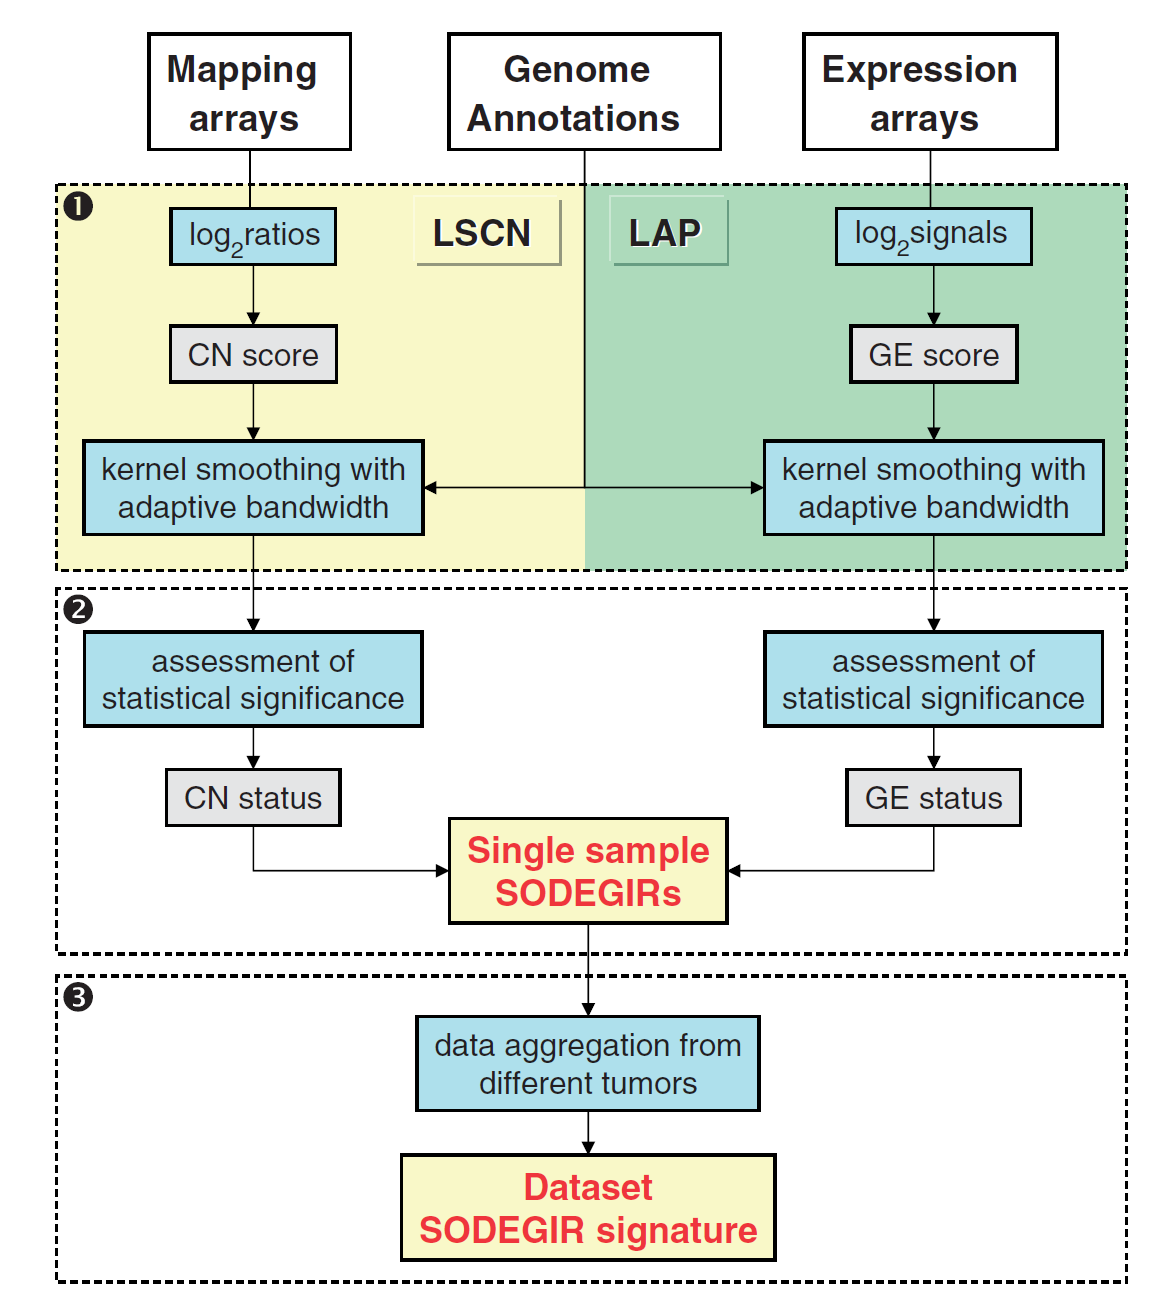
\includegraphics[width=9cm]{images/sodegirWorkflow.png}
  \caption{SODEGIR workflow: workflow for the identification of Significant Overlap of Differentially Expressed and Genomic Imbalanced Regions, as described in \cite{PubMed_19542187}.}
 \label{fig:sodegirWorkflow}
\end{figure}

\paragraph{Sample dataset.} The sample dataset analyzed with SODEGIR procedure is contained in the PREDAsampledata package.
The gene expression dataset is the same described above: the dataset of clear cell renal carcinoma (RCC): ArrayExpress dataset E-TABM-282. The paired copy number data come from ArrayExpress datasets E-TABM-283/E-TABM-284.


\subsubsection{Gene expression data analysis}
% one step function
The function \texttt{SODEGIRpreprocessingGE} allows performing SODEGIR preprocessing of gene expression data starting from RAW cel files with one single function. This function actually performs the same steps of function \texttt{preprocessingGE} but a statistic for each sample is computed: each individual tumor sample is compared with the group of reference normal cells.

\begin{Schunk}
\begin{Sinput}
> SODEGIRGEDataForPREDA <- SODEGIRpreprocessingGE(SampleInfoFile = infofile, 
+     CELfiles_dir = CELfilesPath, custom_cdfname = "gahgu133plus2", 
+     arrayNameColumn = 1, sampleNameColumn = 2, 
+     classColumn = "Class", referenceGroupLabel = "normal", 
+     statisticType = "tstatistic", optionalAnnotations = c("SYMBOL", 
+         "ENTREZID"), retain.chrs = 1:22)
\end{Sinput}
\end{Schunk}

The resulting DataForPREDA object can be immediately analyzed with PREDA\_main function.

\begin{Schunk}
\begin{Sinput}
> SODEGIRGEanalysisResults <- PREDA_main(SODEGIRGEDataForPREDA)
\end{Sinput}
\end{Schunk}


Then from PREDA analysis results, we can extract the list of genomic regions with significant UP or DOWN regulation of gene expression levels.

\begin{Schunk}
\begin{Sinput}
> SODEGIR_GE_UP <- PREDAResults2GenomicRegions(SODEGIRGEanalysisResults, 
+     qval.threshold = 0.05, smoothStatistic.tail = "upper", 
+     smoothStatistic.threshold = 0.5)
> SODEGIR_GE_DOWN <- PREDAResults2GenomicRegions(SODEGIRGEanalysisResults, 
+     qval.threshold = 0.05, smoothStatistic.tail = "lower", 
+     smoothStatistic.threshold = -0.5)
\end{Sinput}
\end{Schunk}

A list of GenomicRegions objects is obtained: with one GenomicRegions object for each sample of the dataset.
Therefore the significant reginons detected in each individual sample can be plotted using genomePlot function: see figure \ref{fig:genomePlotSODEGIRgeOnesample}.


\begin{Schunk}
\begin{Sinput}
> checkplot <- genomePlot(SODEGIRGEanalysisResults, 
+     genomicRegions = c(SODEGIR_GE_UP[1], SODEGIR_GE_DOWN[1]), 
+     grouping = c(1, 1), scale.positions = "Mb", 
+     region.colors = c("red", "blue"))
> title(paste("Sample", names(SODEGIR_GE_UP[1])))
\end{Sinput}
\end{Schunk}

\begin{figure}[htbp]
 \centering
\includegraphics{PREDAtutorial-genomePlotSODEGIRge1}
 \caption{Genome plot for SODEGIR results on gene expression data from one sample.}
 \label{fig:genomePlotSODEGIRgeOnesample}
\end{figure}


Alterantively, a plot representing one single chromosome on multiple samples can be drwan. Figure \ref{fig:genomePlotSODEGIRgeOnechromosome} report a plot for chromsomome 5 across all of the RCC samples: this chromosome is frequently ampliifed in this type of cancer as previuosly discussed \cite{PubMed_19542187}. The custom.labels parameter allow modifying the default chromosomes label on vertical axis.


\begin{Schunk}
\begin{Sinput}
> checkplot <- genomePlot(SODEGIRGEanalysisResults, 
+     genomicRegions = SODEGIR_GE_UP, scale.positions = "Mb", 
+     region.colors = rep("red", times = length(SODEGIR_GE_UP)), 
+     limitChrs = 5, custom.labels = names(SODEGIR_GE_UP))
\end{Sinput}
\end{Schunk}

\begin{figure}[htbp]
 \centering
\includegraphics{PREDAtutorial-genomePlotSODEGIRge2}
 \caption{Genome plot for SODEGIR results on gene expression data for chromosome 5 from all samples.}
 \label{fig:genomePlotSODEGIRgeOnechromosome}
\end{figure}


\subsubsection{Copy number data analysis}
% one step function
Copy number data were obtained with Human Mapping 100K SNP Affymetrix arrays. In particular copy number microarrays data were obtained from a previously described dataset \cite{PubMed_19542187} concerning clear renal cell carcinoma and paired normal diploid cell samples from blood. The initial input copy number data are log-ratio copy number values estimated with CNAG 2.0 software \cite{PubMed_16024607} comparing each tumor samples with paired normal reference from blood.
Copy number data from paired samples are loaded directly from a text file, as well as corresponding annotation, in order to show the general procedure for importing genomics data into PREDA objects from generic sources. First of all the path to the Copy Number data file and annotations is obtained from PREDAsampledata package.

\begin{Schunk}
\begin{Sinput}
> CNdataPath <- system.file("sampledata", "CopyNumber", 
+     package = "PREDAsampledata")
> CNdataFile <- file.path(CNdataPath, "CNAG_data_PREDA.txt")
> CNannotationFile <- file.path(CNdataPath, "SNPAnnot100k.csv")
\end{Sinput}
\end{Schunk}


Then \texttt{StatisticsForPREDAFromfile} function is used to import genomic data from a tab delimited text file into a \texttt{StatisticsForPREDA} object.

\begin{Schunk}
\begin{Sinput}
> CNStatisticsForPREDA <- StatisticsForPREDAFromfile(file = CNdataFile, 
+     ids_column = "AffymetrixSNPsID", testedTail = "both", 
+     sep = "\t", header = TRUE)
\end{Sinput}
\end{Schunk}

Similarly the \texttt{GenomicAnnotationsForPREDAFromfile} function is used to import genomic annotations from a csv file. Please note that different parameters for reading text files can be specified in both functions for reading data from text files, including ``header'', ``sep'', ``quote'', ``na.strings'': these are common parameers used in R function \texttt{read.table()}.

\begin{Schunk}
\begin{Sinput}
> CNGenomicsAnnotationsForPREDA <- GenomicAnnotationsForPREDAFromfile(file = CNannotationFile, 
+     ids_column = 1, chr_column = "Chromosome", 
+     start_column = 4, end_column = 4, strand_column = "Strand", 
+     chromosomesLabelsInput = 1:22, MinusStrandString = "-", 
+     PlusStrandString = "+", optionalAnnotationsColumns = c("Cytoband", 
+         "Entrez_gene"), header = TRUE, sep = ",", 
+     quote = "\"", na.strings = c("NA", "", "---"))
\end{Sinput}
\end{Schunk}

Then genomic data (copy number data) and annotations are merged in to DataForPREDA object.

\begin{Schunk}
\begin{Sinput}
> SODEGIRCNDataForPREDA <- MergeStatisticAnnotations2DataForPREDA(CNStatisticsForPREDA, 
+     CNGenomicsAnnotationsForPREDA, sortAndCleanNA = TRUE, 
+     quiet = FALSE, MedianCenter = TRUE)
\end{Sinput}
\end{Schunk}

A specific aspect of the SODEGIR procedure, is the integration of copy number analysis output with output from GeneExpression data based on the computation of PREDA statistics on the same set of reference positions used for gene expression data. This integration is achieved in the PREDA package by simply providing the annotations for gene expression data as ``outputGenomicAnnotationsForPREDA'' parameter. Please note that genomic annotations for gene expression data are actually included as well into the ``SODEGIRGEDataForPREDA'' object.

\begin{Schunk}
\begin{Sinput}
> SODEGIRCNanalysisResults <- PREDA_main(SODEGIRCNDataForPREDA, 
+     outputGenomicAnnotationsForPREDA = SODEGIRGEDataForPREDA)
\end{Sinput}
\end{Schunk}


Then a list of GenomicRegions objects describing chromosomal regions with altered copy number (gain or loss) can be extracted using \texttt{PREDAResults2GenomicRegions()} function.

\begin{Schunk}
\begin{Sinput}
> SODEGIR_CN_GAIN <- PREDAResults2GenomicRegions(SODEGIRCNanalysisResults, 
+     qval.threshold = 0.01, smoothStatistic.tail = "upper", 
+     smoothStatistic.threshold = 0.1)
> SODEGIR_CN_LOSS <- PREDAResults2GenomicRegions(SODEGIRCNanalysisResults, 
+     qval.threshold = 0.01, smoothStatistic.tail = "lower", 
+     smoothStatistic.threshold = -0.1)
\end{Sinput}
\end{Schunk}

Figure \ref{fig:genomePlotSODEGIRcnOnechromosome} report the genome plot of regions with copy number gain on chromosome 5 across all of the dataset samples.

\begin{Schunk}
\begin{Sinput}
> checkplot <- genomePlot(SODEGIRGEanalysisResults, 
+     genomicRegions = SODEGIR_CN_GAIN, scale.positions = "Mb", 
+     region.colors = rep("red", times = length(SODEGIR_CN_GAIN)), 
+     limitChrs = 5, custom.labels = names(SODEGIR_CN_GAIN))
\end{Sinput}
\end{Schunk}

\begin{figure}[htbp]
 \centering
\includegraphics{PREDAtutorial-genomePlotSODEGIRcn1}
 \caption{Genome plot for SODEGIR results on copy number data for chromosome 5 from all samples.}
 \label{fig:genomePlotSODEGIRcnOnechromosome}
\end{figure}



\subsubsection{SODEGIR procedure}
% overlap
The final integration between gene expression and copy number position related data analysis is achieved by computing the overlap between genomic regions with significant alterations of both types of data. For this purpose it's crucial to analyze the GE and CN data using the same order of samples.

\begin{Schunk}
\begin{Sinput}
> analysesNames(SODEGIRCNanalysisResults)
\end{Sinput}
\begin{Soutput}
 [1] "X27CG"  "X28RA"  "X33BV"  "X36MML" "X37BA"  "X40RR" 
 [7] "X45DM"  "X46SA"  "X47CA"  "X49CA"  "X50PC"  "X51MI" 
\end{Soutput}
\begin{Sinput}
> analysesNames(SODEGIRGEanalysisResults)
\end{Sinput}
\begin{Soutput}
 [1] "X27CG"  "X28RA"  "X33BV"  "X36MML" "X37BA"  "X40RR" 
 [7] "X45DM"  "X46SA"  "X47CA"  "X49CA"  "X50PC"  "X51MI" 
\end{Soutput}
\begin{Sinput}
> all(analysesNames(SODEGIRCNanalysisResults) == 
+     analysesNames(SODEGIRGEanalysisResults))
\end{Sinput}
\begin{Soutput}
[1] TRUE
\end{Soutput}
\end{Schunk}

Then the overlap between up (or down) regulated regions and regions with copy number gain (or loss) is computed for each sample using \texttt{GenomicRegionsFindOverlap()} function.

\begin{Schunk}
\begin{Sinput}
> SODEGIR_AMPLIFIED <- GenomicRegionsFindOverlap(SODEGIR_GE_UP, 
+     SODEGIR_CN_GAIN)
> SODEGIR_DELETED <- GenomicRegionsFindOverlap(SODEGIR_GE_DOWN, 
+     SODEGIR_CN_LOSS)
> names(SODEGIR_AMPLIFIED) <- names(SODEGIR_GE_UP)
> names(SODEGIR_DELETED) <- names(SODEGIR_GE_DOWN)
\end{Sinput}
\end{Schunk}


Figure \ref{fig:genomePlotSODEGIROnechromosome} reports a plot of chromosome 5 SODEGIR for all of the samples.

\begin{Schunk}
\begin{Sinput}
> checkplot <- genomePlot(SODEGIRGEanalysisResults, 
+     genomicRegions = SODEGIR_AMPLIFIED, scale.positions = "Mb", 
+     region.colors = rep("red", times = length(SODEGIR_AMPLIFIED)), 
+     limitChrs = 5, custom.labels = names(SODEGIR_AMPLIFIED))
\end{Sinput}
\end{Schunk}



\begin{figure}[htbp]
 \centering
\includegraphics{PREDAtutorial-genomePlotSODEGIR1}
 \caption{Genome plot for SODEGIR results on chromosome 5 for all samples.}
 \label{fig:genomePlotSODEGIROnechromosome}
\end{figure}


Alterantively we can plot the significant also the regions with significant alterations of gene expression, copy number or SODEGIR from one individual sample: see Figure \ref{fig:genomePlotSODEGIROnesamplefull}.
First of all the selected set of regions is selected from lists containing GenomiRegions objects.

\begin{Schunk}
\begin{Sinput}
> regions_forPlot <- c(SODEGIR_GE_UP[[1]], SODEGIR_CN_GAIN[[1]], 
+     SODEGIR_AMPLIFIED[[1]], SODEGIR_GE_DOWN[[1]], 
+     SODEGIR_CN_LOSS[[1]], SODEGIR_DELETED[[1]])
\end{Sinput}
\end{Schunk}

Then a plot with three copies of each chromosome is drawn (fig.\ref{fig:genomePlotSODEGIROnesamplefull}): each chromosome contains genomic regions of distinct data types as decribed in figure legend.

\begin{Schunk}
\begin{Sinput}
> checkplot <- genomePlot(SODEGIRGEanalysisResults, 
+     genomicRegions = regions_forPlot, grouping = c(1:3, 
+         1:3), scale.positions = "Mb", region.colors = c("red", 
+         "red2", "red4", "blue", "blue2", "blue4"))
> legend(x = 1.4e+08, y = 22 * 3, legend = c("GeneExpression UP", 
+     "CopyNumber gain", "SODEGIR amplified", "GeneExpression DOWN", 
+     "CopyNumber loss", "SODEGIR deleted"), fill = c("red", 
+     "red2", "red4", "blue", "blue2", "blue4"))
> title(paste("Sample", names(SODEGIR_GE_UP[[1]])))
\end{Sinput}
\end{Schunk}



\begin{figure}[htbp]
 \centering
\includegraphics{PREDAtutorial-genomePlotSODEGIR2}
 \caption{Genome plot for SODEGIR results on one sample, including copy number and gene expression results on distinct lines.}
 \label{fig:genomePlotSODEGIROnesamplefull}
\end{figure}


\subsubsection{Dataset signature}
% dataset signature
The final step of SODEGIR analysis is the evaluation of a dataset level signature for recurrent SODEGIRs across multiple samples.
This step is performed using function \texttt{computeDatasetSignature()} that requires as input a set of reference genomic annotations (derived from ``GEDataForPREDA'' object) and the list of SODEGIRs from all of hte dataset samples.

\begin{Schunk}
\begin{Sinput}
> SDGsignature_amplified <- computeDatasetSignature(GEDataForPREDA, 
+     genomicRegionsList = SODEGIR_AMPLIFIED)
> SDGsignature_deleted <- computeDatasetSignature(GEDataForPREDA, 
+     genomicRegionsList = SODEGIR_DELETED)
\end{Sinput}
\end{Schunk}

The significance of recurrent amplified and deleted regions is computed independently as above shown.
The significantly recurrent SODEGIR (i.e. the dataset SDG signature) can be plotted on the genome as well.

\begin{Schunk}
\begin{Sinput}
> checkplot <- genomePlot(SODEGIRGEanalysisResults, 
+     genomicRegions = c(SDGsignature_amplified, 
+         SDGsignature_deleted), grouping = c(1, 
+         1), scale.positions = "Mb", region.colors = c("red", 
+         "blue"))
\end{Sinput}
\end{Schunk}


\begin{figure}[htbp]
 \centering
\includegraphics{PREDAtutorial-genomePlotSODEGIRsignature}
 \caption{Genome plot for SODEGIR signature over the entire dataset.}
 \label{fig:genomePlotSODEGIRsignature}
\end{figure}


Alternatively the significant regions can be visualized as a dataframe using the function \texttt{GenomicRegions2dataframe()}.

\begin{Schunk}
\begin{Sinput}
> GenomicRegions2dataframe(SDGsignature_amplified[[1]])
\end{Sinput}
\begin{Soutput}
  chr     start       end
1   5  61727796  69763306
2   5  99924642 102632300
3   5 111784012 159572636
4   5 169467401 180618352
5   7  34985892  34985892
6   7  36233519  39671965
7   7 105694420 106087606
\end{Soutput}
\begin{Sinput}
> GenomicRegions2dataframe(SDGsignature_deleted[[1]])
\end{Sinput}
\begin{Soutput}
  chr    start      end
1   3 35734922 58856766
\end{Soutput}
\end{Schunk}

\section{General remarks}
The PREDA package implements an informatic infrastructure to perform position related analysis of genomics data. The sample analyses reported in this tutorial just considered few samples possible applications of this procedure. The availability of multiple parameters for data smoothing and for all of the other steps of the procedure allows the adoption of PREDA to address several distinct biological problems. The SODEGIR procedure itself could be actually used to integrate analyses of different combinations of genomics data. PREDA package is therefore built to constitute a generalized approach for position related data analysis for functional genomics applications.


\newpage
\addcontentsline{toc}{section}{References}
\bibliographystyle{unsrt}
\bibliography{PREDA}


\end{document}

